\section{Introduction}

Chapter \ref{chp:case_overview} described each of the three cases and contrasted these in terms of their maturity, type of open innovation, demographics, and different knowledge provider ties. The three cases are quite different in terms of the nature of open innovation (vis-\`a-vis inbound, outbound, and coupled open innovation), their maturity, geographic spread of participants, and extent of tacit and explicit knowledge exchanges. \medskip

This chapter presents the results of our exponential random graph modelling. Recall from Chapter \ref{chp:methodology} that mixing quantitative and qualitative methods is challenging because of the complex ontological and epistemological issues involved. The stratified ontology of critical realism allows for the legitimate combination of qualitative and quantitative methods. From a critical realist perspective, the exponential random graph models address observed or experienced reality, i.e. the knowledge sharing events in each case. The modelling identifies which network configurations can explain the global structure of observed networks. It targets social processes or mechanisms referred to in the seven propositions developed in Chapter \ref{chp:lit_review}. \medskip

Two sets of modelling were done. The first set examined the role of motivation, trust, and power in tacit and explicit knowledge exchanges in each case and across all three cases (see Section \ref{sec:motivation} for the rationale for this). Our second set of models examined the significance of different broker roles in each case (refer to Section \ref{sec:brokerage} for a description of these roles). Recall that the online survey asked respondents to name others who provided them with valuable and relevant knowledge. As explained in the section on data pre-processing in Chapter \ref{chp:methodology}, ties were reversed to depict named knowledge providers as senders of knowledge. Reversing the ties ensures we portray the actual direction of knowledge flows. \medskip

\begin{sidewaystable}[]
\tiny
\centering
\caption[Rationale for ERGM parameters]{Rationale for ERGM parameters used in this study. Refer to Table \ref{tab:ergm_params} for more detail about the parameters.}
\label{tab:prop_pars}
\resizebox{\textwidth}{!}{%
\begin{tabular}{p{0.5cm} p{6cm} p{6cm} p{8cm}}
\toprule
\multicolumn{1}{c}{Proposition} & \multicolumn{1}{c}{Statement} & \multicolumn{1}{c}{Model parameter} & \multicolumn{1}{c}{Rationale} \\ \midrule
\multirow[t]{8}{=}{1a} & \multirow[t]{8}{=}{Open innovation requires practitioners to connect across organisational and disciplinary boundaries so that they can transfer and apply their know-how and know-what in novel ways.} & Reciprocity (mutuality) & Participants are expected to exchange knowledge in a collaboration. \\
& & AT-T (path closure) & Network closure indicates knowledge is being assimilated and applied in practice within local groups. \\
& & Employer (match) & A significant and positive match effect indicates much of the knowledge is being shared internally. \\
& & Employer (mismatch reciprocity) & A significant mismatch reciprocity effect indicates knowledge sharing is reciprocated across organisational boundaries. \\
& & $b_{IO}$ (representative broker) & An indicator of knowledge outflows across organisational boundaries. \\
& & $b_{OI}$ (gatekeeper) & An indicator of knowledge inflows across organisational boundaries. \\
& & $b_O$ (liaison role) & Brokers are ensuring knowledge is passed onto two third parties. \\
& & $w_O$ (itinerant broker) & Brokers facilitate knowledge sharing between disconnected actors from the same organisation. \\ \midrule
\multirow[t]{4}{=}{1b} & \multirow[t]{4}{=}{Reducing cognitive distance between open innovation partners requires significant social interaction to support learning and the application of knowledge in practice.} & AT-T (path closure) & Network closure indicates knowledge is being assimilated and applied in practice within local groups. \\
& & Reciprocity (mutuality) & Participants are engaged in mutual learning. \\
& & AinS (popularity spread) & Participants are gravitating to knowledgeable people in the partnership. \\
& & AoutS (activity spread) & Knowledgeable participants are sharing their knowledge widely. \\ \midrule
\multirow[t]{6}{=}{2a} & \multirow[t]{6}{=}{Successful open innovation requires deliberate brokerage actions that lead to network closure.} & A2P-T (multiple connectivity) & A small number of actors are helping connect multiple disconnected actors (possible evidence of tertius iungens and conduit brokerage). \\
& & $b_{OI}$ (gatekeeper) & Partners are benefiting from knowledge inflows. \\
& & $b_{IO}$ (representative broker) & Partners are sharing knowledge with other partners. \\
& & $b_O$ (liaison role) & Partners ensure other parties benefit from knowledge sharing. \\
& & $w_O$ (itinerant broker) & External partner is helping resolve internal disconnects. \\
& & $w_I$ (internal coordinator) & Knowledge is being socialised internally. \\ \midrule
3a & Formal structures inhibit tacit knowledge exchange in open innovation partnerships. & Reporting hierarchy (dyadic covariate) & Knowledge flows aligned with formal reporting structures. \\ \midrule
\multirow[t]{6}{=}{3b} & \multirow[t]{6}{=}{Innate needs and subjective norms moderate individual willingness to seek out or share tacit knowledge.} &
Autonomous motivation (sender) & Participants enjoy sharing their knowledge with others. \\
& & Autonomous motivation (receiver) & Participants develop their competence or sense of self-efficacy by seeking knowledge from others. \\
& & Controlled motivation (sender) & Participants feel obliged to share their knowledge. \\
& & Controlled motivation (receiver) & Participants feel obliged to obtain knowledge from others. \\
& & Identification with group (sender) & Participants who identify strongly with their group are less inclined to share their knowledge with third-parties. \\
& & Identification with group (receiver) & Participants who identify strongly with their group are less likely to receive knowledge from third-parties. \\ \midrule
\multirow[t]{3}{=}{4a} & \multirow[t]{3}{=}{Reciprocity and closure in tacit knowledge exchange networks indicate high levels of trust in open innovation partnerships.} & Reciprocity (mutuality) & Participants are unlikely to exchange knowledge with each other in a low-trust setting. \\
& & AT-T (path closure) & Network closure indicates knowledge is being exchanged in close-knit groups. \\
& & Employer (mismatch reciprocity) & One expects knowledge sharing to be reciprocated between partners in a high-trust setting. \\ \midrule
4b & Who people choose to empower with their know-how depends on how much they trust the receiver to use their know-how in mutually beneficial ways. & Cognition-based trust (dyadic covariate) & People are more likely to share knowledge with people they trust. \\ \bottomrule
\end{tabular}%
}
\end{sidewaystable}

\section{Models exploring motivation, trust and power}

The first set of models examined how autonomous motivation, cognition-based trust, and reporting hierarchy shape tacit and explicit knowledge sharing ties. Apart from modelling each case separately, the different network layers from each case were combined and modelled as one big network. As explained in Chapter \ref{chp:methodology} (Section \ref{sec:stat_network}), the case-specific networks are non-overlapping and are separated by structural zeros. Only within-case ties, and not between-case ties, are modelled \citep{lusher2012trust}. The assumption is that the same endogenous and exogenous processes operate across all three cases \citep{kalish2013brain}. Modelling all the networks together in one ERGM allows us to identify which social processes stand out more generally. \medskip

Parameters used in the first set of models included controlled and autonomous sender/receiver effects (to determine to what extent the two types of motivation predict knowledge sharing) and cognition-based trust and reporting hierarchy dyadic covariate effects (to check to what extent knowledge sharing ties align with cognition-based trust ties and reporting hierarchy ties). Other parameters controlled for network structure (reciprocity, simple and multiple connectivity, popularity and activity spread, and transitive closure), homophily (age and education level difference, employer match), personality (openness to experience sender/receiver), social identity (identification with group sender/receiver), reciprocal exchanges across organisational boundaries (employer mismatch reciprocity), and geographic proximity (log of kilometre distance). Table \ref{tab:prop_pars} shows how specific parameters relate to the propositions. The choice of actor-relation effects to include in the first set of models was guided by a correlation analysis of survey response items. Figure \ref{fig:corr_analysis} is a correlation matrix showing which survey response items are positively or negatively correlated with each other. Care was taken not to include highly correlated items in the models. For example, identification with the collaboration, one's employer organisation, or team are highly correlated. Hence, only identification with team (group) was included as a model parameter. The six items from the work motivation scale were aggregated into controlled and autonomous motivation to mitigate item correlation. Results for each case are presented side-by-side in Table \ref{tab:ergm_1}. Table \ref{tab:ergm_2} presents the results of the combined network analysis. \medskip

\begin{figure}
    \centering
    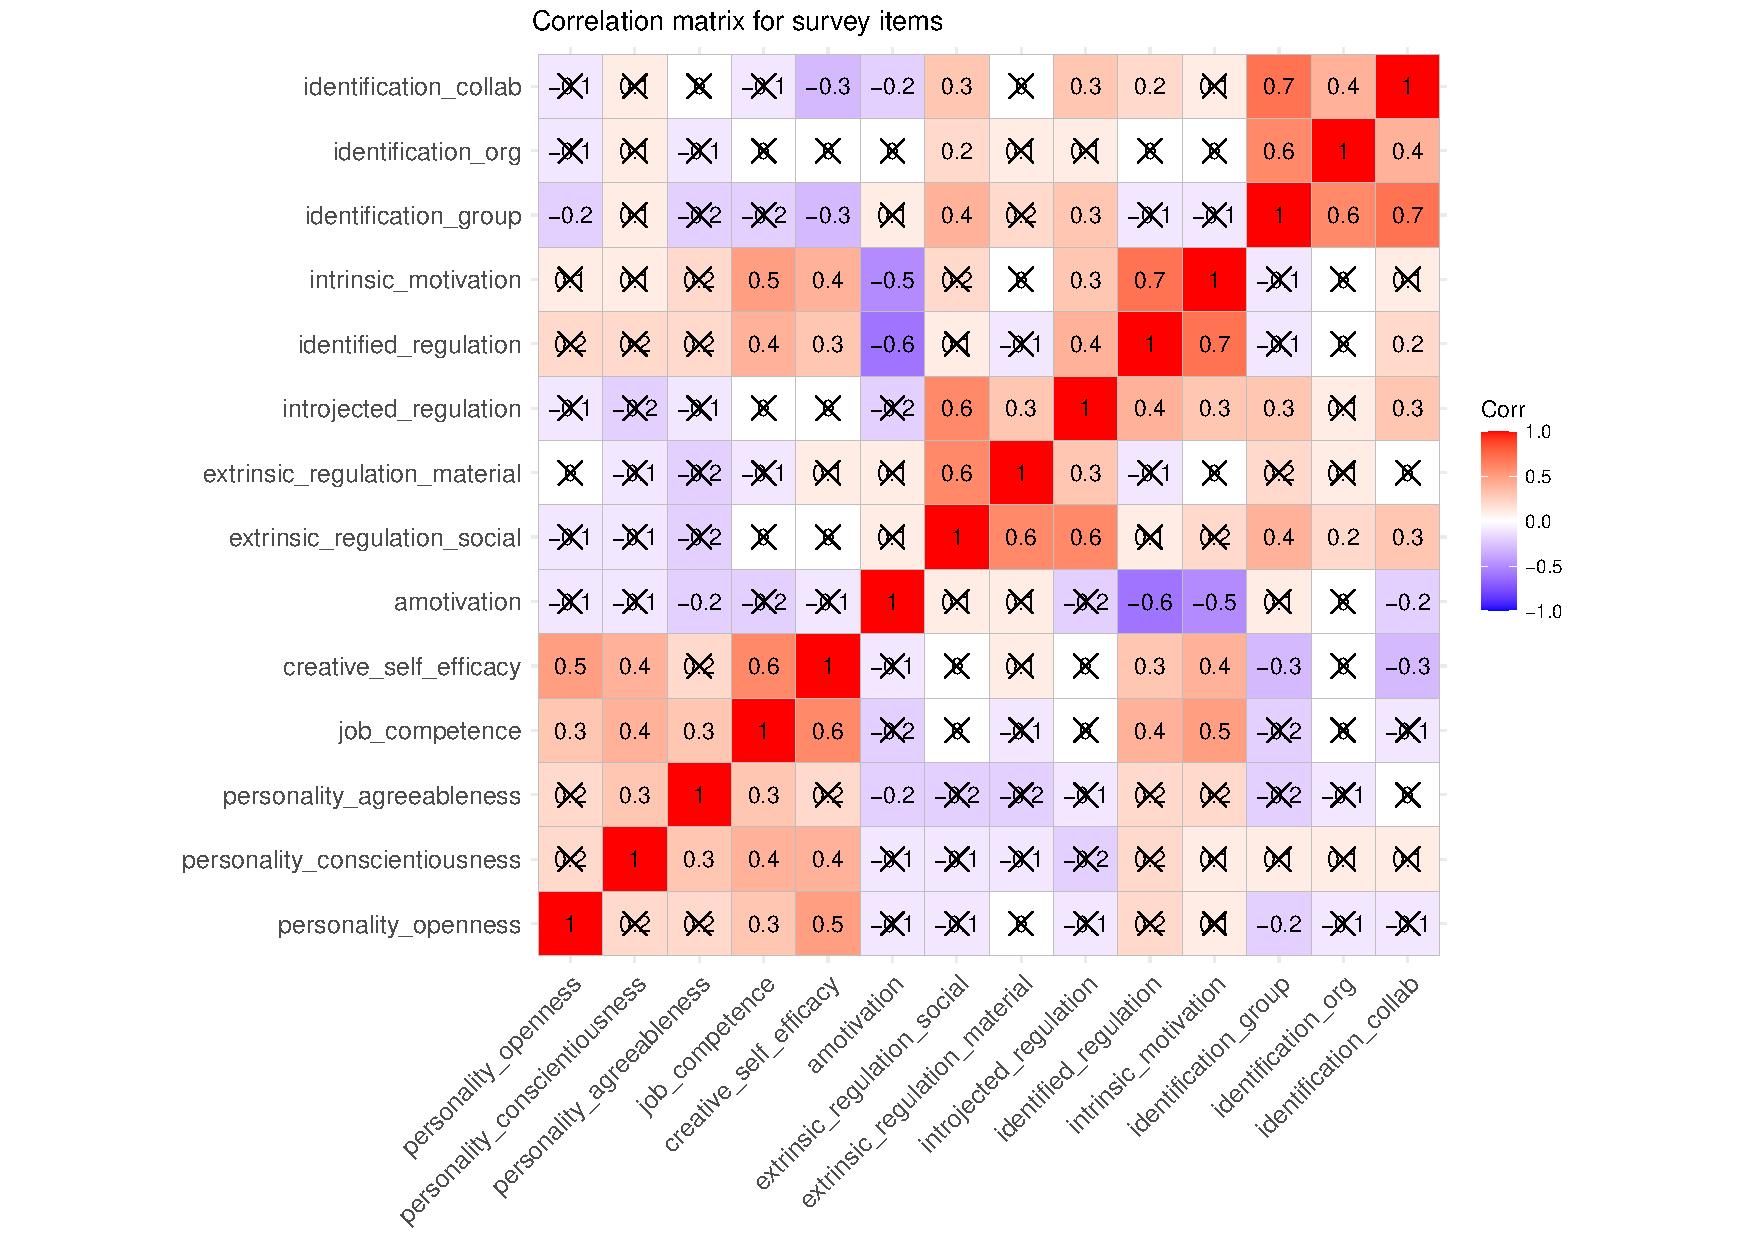
\includegraphics[width = \textwidth]{Images/corr_plot.pdf}
    \caption[Correlation between survey response items]{Correlation between survey response items. The crosses mark non-significant correlation effects.}
    \label{fig:corr_analysis}
\end{figure}

\begin{sidewaystable}[p]
\centering
\resizebox{0.9\textwidth}{!}{%	
\begin{threeparttable}
\footnotesize
\setlength{\tabcolsep}{6pt}
\renewcommand{\arraystretch}{1}
\caption[Parameter estimates for the first set of ERGMs]{ERGM parameter estimates for models exploring motivation, trust and power in tacit and explicit knowledge provider networks. Refer to Table \ref{tab:ergm_params} for an explanation of network parameters.}
\label{tab:ergm_1}
\begin{tabular}{@{}lrrcrrcrr@{}}
\toprule
& \multicolumn{2}{c}{Case 1} &  & \multicolumn{2}{c}{Case 2} &  & \multicolumn{2}{c}{Case 3} \\ \cmidrule(lr){2-3} \cmidrule(lr){5-6} \cmidrule(l){8-9} \multicolumn{1}{c}{} & \multicolumn{1}{c}{Tacit} & \multicolumn{1}{c}{Explicit} & \multicolumn{1}{c}{} & \multicolumn{1}{c}{Tacit} & \multicolumn{1}{c}	{Explicit} & \multicolumn{1}{c}{} & \multicolumn{1}{c}{Tacit} & \multicolumn{1}{c}{Explicit} \\
\cmidrule(lr){2-3} \cmidrule(lr){5-6} \cmidrule(l){8-9} 
\textbf{Purely structural effects (endogenous)} & \multicolumn{1}{l}{} & \multicolumn{1}{l}{} &  & \multicolumn{1}{l}{} & \multicolumn{1}{l}{} &  & \multicolumn{1}{l}{} & \multicolumn{1}{l}{} \\
Arc (edge) & -16.13 (4.39)* & 9.41 (7.03)\phantom{*} &  & -4.59 (1.4)* & -3.73 (1.94)\phantom{*} &  & -7.33 (1.47)* & -2.41 (1.21)\phantom{*} \\
Reciprocity (mutuality) & -1.76 (1.29)\phantom{*} & -2.04 (1.19)\phantom{*} &  & -0.3 (0.65)\phantom{*} & -0.16 (0.93)\phantom{*} &  & -0.45 (0.62)\phantom{*} & -0.75 (0.46)\phantom{*} \\
TwoPath (simple connectivity) & -2.63 (1.60)\phantom{*} & -0.25 (0.24)\phantom{*} &  & -0.01 (0.03)\phantom{*} & 0.08 (0.07)\phantom{*} &  & -0.24 (0.13)\phantom{*} & -0.26 (0.13)* \\
AinS (popularity spread) & -0.87 (0.73)\phantom{*} & 1.82 (0.65)* &  & 0.02 (0.42)\phantom{*} & 0.67 (0.38)\phantom{*} &  & 0.57 (0.34)\phantom{*} & 0.45 (0.29)\phantom{*} \\
AoutS (activity spread) & 0.21 (0.57)\phantom{*} & -5.96 (2.79)* &  & 0.71 (0.40)\phantom{*} & -0.74 (0.80)\phantom{*} &  & 0.89 (0.37)* & 0.36 (0.31)\phantom{*} \\
AT-T (path closure) & 1.93 (0.73)* & 0.50 (0.37)\phantom{*} &  & 0.73 (0.23)* & 0.14 (0.20)\phantom{*} &  & 0.49 (0.26)\phantom{*} & 0.49 (0.25)\phantom{*} \\
A2P-T (multiple connectivity) & 2.58 (1.61)\phantom{*} & 0.37 (0.28)\phantom{*} &  & -0.22 (0.06)* & -0.06 (0.1)\phantom{*} &  & 0.35 (0.13)* & 0.36 (0.14)* \\ \\
\textbf{Actor-relation effects (exogenous)} & \multicolumn{1}{l}{} & \multicolumn{1}{l}{} &  & \multicolumn{1}{l}{} & \multicolumn{1}{l}{} &  & \multicolumn{1}{l}{} & \multicolumn{1}{l}{} \\
Age (difference) & 0.03 (0.04)\phantom{*} & -0.01 (0.02)\phantom{*} &  & 0.00 (0.01)\phantom{*} & 0.00 (0.01)\phantom{*} &  & -0.01 (0.02)\phantom{*} & -0.04 (0.01)* \\
Education level (difference) & -0.34 (0.23)\phantom{*} & 0.18 (0.13)\phantom{*} &  & 0.08 (0.07)\phantom{*} & -0.07 (0.08)\phantom{*} &  & -0.12 (0.11)\phantom{*} & -0.12 (0.11)\phantom{*} \\
Work experience (sender) & 0.00 (0.05)\phantom{*} & -0.12 (0.08)\phantom{*} &  & 0.02 (0.01)* & 0.02 (0.02)\phantom{*} &  & -0.02 (0.02)\phantom{*} & -0.05 (0.02)* \\
Job tenure (sender) & 0.06 (0.06)\phantom{*} & 0.18 (0.09)* &  & 0.00 (0.01)\phantom{*} & -0.01 (0.02)\phantom{*} &  & 0.04 (0.02)\phantom{*} & 0.07 (0.03)* \\
Openness (sender) & 1.19 (2.29)\phantom{*} & -3.92 (3.85)\phantom{*} &  & -0.35 (0.47)\phantom{*} & 0.13 (0.92)\phantom{*} &  & 0.06 (0.63)\phantom{*} & -0.46 (0.68)\phantom{*} \\
Openness (receiver) & 6.19 (2.58)* & -0.66 (1.29)\phantom{*} &  & -0.18 (0.67)\phantom{*} & 0.2 (0.69)\phantom{*} &  & -1.08 (0.64)\phantom{*} & 0.61 (0.59)\phantom{*} \\
Controlled motivation (sender) & -0.89 (1.88)\phantom{*} & -12.22 (4.84)* &  & 0.56 (0.68)\phantom{*} & 2.16 (1.34)\phantom{*} &  & 2.84 (1.01)* & 1.25 (0.85)\phantom{*} \\
Controlled motivation (receiver) & -2.44 (2.90)\phantom{*} & 1.61 (1.42)\phantom{*} &  & -1.53 (0.84)\phantom{*} & -1.23 (0.93)\phantom{*} &  & -2.69 (0.94)* & 0.67 (0.71)\phantom{*} \\
Autonomous motivation (sender) & 1.80 (2.12)\phantom{*} & -0.67 (2.32)\phantom{*} &  & 0.21 (0.52)\phantom{*} & -1.93 (1.11)\phantom{*} &  & -0.24 (0.88)\phantom{*} & -1.08 (0.7)\phantom{*} \\
Autonomous motivation (receiver) & 9.35 (3.03)* & -1.22 (1.12)\phantom{*} &  & 1.53 (0.75)* & 1.61 (0.90)\phantom{*} &  & 3.62 (1.12)* & -0.15 (0.69)\phantom{*} \\
Identification with group (sender) & 0.13 (1.13)\phantom{*} & -0.36 (1.54)\phantom{*} &  & 0.00 (0.33)\phantom{*} & 1.77 (0.79)* &  & -1.19 (0.48)* & -0.1 (0.42)\phantom{*} \\
Identification with group (receiver) & 2.05 (1.62)\phantom{*} & -0.91 (0.77)\phantom{*} &  & 0.02 (0.47)\phantom{*} & -0.08 (0.38)\phantom{*} &  & -0.08 (0.42)\phantom{*} & -0.11 (0.39)\phantom{*} \\
Employer (match) & 0.07 (0.86)\phantom{*} & 2.36 (0.89)* &  & 0.77 (0.32)* & 0.64 (1.05)\phantom{*} &  & 0.61 (0.35)\phantom{*} & 0.46 (0.31)\phantom{*} \\
Employer (mismatch reciprocity) & -8.74 (22.83)\phantom{*} & 3.79 (1.32)* &  & 0.71 (0.68)\phantom{*} & 0.48 (0.26)\phantom{*} &  & 1.92 (0.83)* & -0.42 (1.21)\phantom{*} \\ \\
\textbf{Dyadic covariate effects (exogenous)} & \multicolumn{1}{l}{} & \multicolumn{1}{l}{} &  & \multicolumn{1}{l}{} & \multicolumn{1}{l}{} &  & \multicolumn{1}{l}{} & \multicolumn{1}{l}{} \\
Cognition-based tust & 2.75 (0.79)* & 2.53 (0.56)* &  & 0.78 (0.21)* & 0.96 (0.40)* &  & 1.47 (0.33)* & 0.34 (0.28)\phantom{*} \\
Reporting hierarchy & 0.47 (0.81)\phantom{*} & 0.31 (0.68)\phantom{*} &  & -1.02 (0.48)* & -0.01 (0.05)\phantom{*} &  & 0.62 (0.50)\phantom{*} & 0.84 (0.4)* \\
Geographic proximity & -0.26 (0.13)* & 0.08 (0.09)\phantom{*} &  & 0.00 (0.04)\phantom{*} & 0.00 (0.00)\phantom{*} &  & -0.08 (0.05)\phantom{*} & -0.22 (0.05)* \\ \bottomrule
\end{tabular}

\begin{tablenotes}
\footnotesize
\item[a] Estimates are significant (*) when the absolute value of the parameter estimate is more than twice the magnitude of the estimated standard error.
\item[b] Goodness of fit scores for non-explicitly modelled statistics were less than 2 in all models, a, and less than 0.1 for all explicitly modelled effects, indicating the models provide adequate fit to most aspects of the social structure.

\end{tablenotes}

\end{threeparttable}
%
}
\end{sidewaystable}

\subsection{Case 1}

Looking at the results for Case 1, parameter estimates for the tacit knowledge provider network show significant and positive effects for path closure (AT-T = 1.93), openness to experience (receiver = 6.19), autonomous motivation (receiver = 9.35), and cognition-based trust (dyadic covariate = 2.75). These effects suggest participants prefer to share their tacit knowledge with others they have strong ties with. The significant and positive receiver effects reflect a strong learning orientation, i.e. participants who are open to experience or autonomously motivated are more likely to seek out tacit knowledge. The significant and negative effect observed for geographic proximity (dyadic covariate = -0.26) indicates that tacit knowledge is more likely to be exchanged with others who are nearby. The negative parameter estimate represents less distance between network actors. \medskip

As to the explicit knowledge provider network, parameter estimates show significant and positive effects for popularity spread (AinS = 1.82), job tenure (sender = 0.18), employer (match = 2.36 and mismatch reciprocity = 3.79), and cognition-based trust (dyadic covariate = 2.53). The popularity spread effect indicates that participants are more likely to direct explicit knowledge to a few actors only. Explicit knowledge tends to be provided by participants who have been in their current job for some time (significant and positive job tenure (sender) effect). The employer (match) effect indicates a tendency to direct explicit knowledge to others from the same organisation. That there is also a significant two-way exchange of explicit knowledge across organisational boundaries (employer (mismatch reciprocity)) is a sign of good collaboration. The significant and negative effect for activity spread suggests explicit knowledge is being evenly distributed and not provided to a few select individuals. Moreover, the significant and negative controlled motivation (sender) effect (-12.22) suggests that controlled motivation leads to significant less explicit knowledge sharing. Formal structure is not significant in the explicit knowledge provider network for Case 1. This suggests that formal structure is not aligned with explicit knowledge sharing

\subsection{Case 2}

Modelling of the tacit knowledge provider network yields significant and positive effects for path closure (AT-T = 0.73), work experience (sender = 0.02), autonomous motivation (receiver = 1.53), and cognition-based trust (dyadic covariate = 0.78). The effects for path closure indicates that participants in Case 2 are likely to share tacit knowledge with others in the local neighbourhood of their network. Moreover, the effect for cognition-based trust indicates participants prefer to share their tacit knowledge with others they trust. Recipients of tacit knowledge also tend to be autonomously motivated. This suggests they have a strong learning orientation. There are significant and negative effects for both multiple connectivity (A2P-T = -0.22) and reporting hierarchy (dyadic covariate = -1.02). The combination of a significant and positive effect for path closure and a significant and negative effect for multiple connectivity is a sign of good collaboration, suggesting paths of knowledge sharing are shortened by closing paths into triangles, thus short-cutting knowledge sharing paths. Participants are sufficiently well-connected that there is little brokerage in the knowledge sharing network. The significant and negative effect for reporting hierarchy indicates that tacit knowledge sharing happens mostly through informal structures. Geographic proximity is not a significant factor in the tacit knowledge provider network. \medskip

With respect to the explicit knowledge provider network, the parameter estimates only show significant and positive effects for identification with group (sender = 1.77) and cognition-based trust (dyadic covariate = 0.96). Explicit knowledge is more likely to be provided by those who identify strongly with the group, and to others who are trusted.

\subsection{Case 3}

Parameter estimates for the tacit knowledge provider network show significant and positive effects for activity spread (AoutS = 0.89), multiple connectivity (A2P-T = 0.35), controlled motivation (sender = 2.81), autonomous motivation (receiver = 3.62), employer (mismatch reciprocity = 1.92), and cognition-based trust (dyadic covariate = 1.47). The significant and positive effect for activity spread suggests tacit knowledge is being provided by a relatively small number of participants. Put differently, just a few individuals are providing most of the expertise in this case. Participants are also more likely to share their tacit knowledge with others they trust. The significant and positive effect for multiple connectivity is an indicator of substantial brokerage. This is not too surprising, given the open innovation partnership was relatively new and people were still getting to know each other. As with the other cases, recipients of tacit knowledge tend to be autonomously motivated. The significant and positive effect for controlled motivation (sender) suggests, contrary to expectations, that many participants feel obliged to share their tacit knowledge. There is a significant two-way exchange of tacit knowledge across organisational boundaries, indicated by the significant and positive effect for employer (mismatch reciprocity). \medskip

As this case is about providing an innovative web-based data analysis platform, we expect explicit knowledge to feature strongly. The parameter estimates for the explicit knowledge provider network show significant and positive effects for multiple connectivity (A2P-T = 0.36), job tenure (sender = 0.07), and reporting hierarchy (dyadic covariate = 0.84). In other words, much of the explicit knowledge flowing through the network is coming from participants who have been in their job for some time. Explicit knowledge also tends to flow up the reporting hierarchy. The estimates show significant and negative effects for simple connectivity (TwoPath = -0.26), age (difference = -0.04), work experience (sender = -0.05), and geographic proximity (dyadic covariate = -0.22). These indicate that received explicit knowledge is not passed on in simple brokerage structures (although the multiple connectivity (A2P-T) effect indicates multiple brokerage structures are present). Age homophily is a factor in explicit knowledge exchanges, and more experienced participants are less likely to share explicit knowledge with others, i.e. participants who share more explicit knowledge tend to have less experience. Explicit knowledge is also more likely to be exchanged with geographically proximate participants. \medskip

\begin{table}[hbt!]
\centering
\resizebox{0.9\textwidth}{!}{	
\begin{threeparttable}
\footnotesize
\setlength{\tabcolsep}{6pt}
\renewcommand{\arraystretch}{1}
\caption{ERGM parameter estimates for the combined tacit and explicit knowledge provider networks.}
\label{tab:ergm_2}
\begin{tabular}{@{}lrlr@{}}
\toprule
 & \multicolumn{3}{c}{Cases 1 + 2 + 3} \\ \cmidrule(l){2-4} 
 & \multicolumn{1}{c}{Tacit} &  & \multicolumn{1}{c}{Explicit} \\ \cmidrule(lr){2-2} \cmidrule(l){4-4} 
\textbf{Purely structural effects (endogenous)} &  &  &  \\
Arc (edge) & -4.66 (0.71)* &  & -2.95 (0.83)* \\
Reciprocity (mutuality) & -0.37 (0.39)\phantom{*} &  & -0.51 (0.37)\phantom{*} \\
TwoPath (simple connectivity) & -0.05 (0.04)\phantom{*} &  & -0.09 (0.06)\phantom{*} \\
AinS (popularity spread) & 0.01 (0.18)\phantom{*} &  & 0.63 (0.19)* \\
AoutS (activity spread) & 0.63 (0.18)* &  & 0.05 (0.21)\phantom{*} \\
AT-T (path closure) & 0.84 (0.17)* &  & 0.56 (0.13)* \\
A2P-T (multiple connectivity) & 0.01 (0.05)\phantom{*} &  & 0.09 (0.08)\phantom{*} \\
&  &  &  \\
\textbf{Actor-relation effects (exogenous)} &  &  &  \\
Age (difference) & -0.01 (0.01)\phantom{*} &  & -0.01 (0.01)\phantom{*} \\
Education level (difference) & 0.08 (0.04)* &  & 0.03 (0.04)\phantom{*} \\
Work experience (sender) & 0.00 (0.01)\phantom{*} &  & -0.01 (0.01)\phantom{*} \\
Job tenure (sender) & 0.00 (0.01)\phantom{*} &  & 0.01 (0.01)\phantom{*} \\
Openness (sender) & -0.53 (0.34)\phantom{*} &  & -0.33 (0.41)\phantom{*} \\
Openness (receiver) & -0.31 (0.39)\phantom{*} &  & 0.20 (0.32)\phantom{*} \\
Controlled motivation (sender) & 0.55 (0.57)\phantom{*} &  & 0.56 (0.62)\phantom{*} \\
Controlled motivation (receiver) & -0.76 (0.64)\phantom{*} &  & -0.32 (0.48)\phantom{*} \\
Autonomous motivation (sender) & -0.62 (0.39)\phantom{*} &  & -1.29 (0.44)* \\
Autonomous motivation (receiver) & 1.71 (0.54)* &  & 0.12 (0.39)\phantom{*} \\
Identification with group (sender) & 0.08 (0.23)\phantom{*} &  & 0.14 (0.27)\phantom{*} \\
Identification with group (receiver) & -0.32 (0.25)\phantom{*} &  & 0.25 (0.22)\phantom{*} \\
Employer (match) & 0.47 (0.16)* &  & 0.49 (0.16)* \\
Employer (mismatch reciprocity) & 0.77 (0.46)\phantom{*} &  & 1.07 (0.45)* \\
 &  &  &  \\
\textbf{Dyadic covariate effects (exogenous)} &  &  &  \\
Cognition-based trust & 1.26 (0.16)* &  & 0.89 (0.16)* \\
Reporting hierarchy & 0.30 (0.24)\phantom{*} &  & 0.82 (0.22)* \\
Geographic proximity & 0.00 (0.02)\phantom{*} &  & -0.07 (0.02)* \\ \bottomrule
\end{tabular}
    \begin{tablenotes}
      \small
      \item Estimates are significant (*) when the absolute value of the parameter estimate is more than twice the magnitude of the estimated standard error.
      \item Goodness of fit scores were less than 2 for more than 97.85\% of the non-explicitly modelled statistics, indicating the models adequately fit most aspects of the knowledge exchange structure
    \end{tablenotes}
\end{threeparttable}
}
\end{table}

\subsection{Combined network}

As mentioned earlier, the combined network analysis allows us to identify which social processes are common across all three cases. Parameter estimates for the combined tacit knowledge network show a significant and positive effect for activity spread and path closure (0.63 and 0.84, respectively). From this one can infer that there are a few knowledgeable people who are happy to share their know-how with others. Much of this know-how is shared with other members of their workgroup. The significant and positive employer (match) effect (0.47) indicates that people are also more likely to share their tacit knowledge with others employed in the same organisation. The significant and positive effect for education level difference (difference = 0.08) indicates that tacit knowledge tends to be exchanged between actors with different education levels (there is a heterophily effect for education level). We also see a significant and positive autonomous motivation (receiver) effect (1.71) that indicates that recipients of tacit knowledge tend to be autonomously motivated. People also tend to share their know-how with others they deem trustworthy (significant and positive cognition-based trust dyadic covariate effect = 1.26). \medskip

In contrast, parameter estimates for the combined explicit knowledge provider network show a significant and positive effect for popularity spread (0.63), indicating that there is a general tendency for explicit knowledge to flow to a small number of individual actors in the network. Moreover, the significant and positive dyadic covariate effect for reporting hierarchy in the explicit knowledge provider network (0.82) indicates that across the three case studies, people are quite likely to provide explicit knowledge to their bosses. Like the combined tacit knowledge provider network, there is a significant and positive transitive path closure effect (0.56) that suggests explicit knowledge is more likely to be shared with others belonging in one's local neighbourhood of knowledge sharing connections. Remember, transitive path closure is the \enquote{closure} of a two-path brokerage tie and in addition to knowledge flowing from person A to B and then onto person C, the path closure also adds a direct path from A to C (i.e. a shortcut that allows knowledge to get directly to where it might be required). Interestingly, the significant and negative autonomous motivation (sender) effect (-1.29) indicates that autonomously motivated people are generally less likely to share explicit knowledge. One may infer autonomously motivated individuals do not feel pressured to share explicit knowledge. As with the combined tacit knowledge provider network, explicit knowledge tends to be shared with others employed by the same organisation (significant and positive employer (match) effect = 0.49). However, the significant and positive employer (mismatch reciprocity) effect (1.07) indicates that explicit knowledge exchanges among open innovation partners tend to be reciprocal. People are also inclined to share explicit knowledge with people they trust (significant and positive dyadic cognition-based trust covariate effect = 0.89) and who are nearby (significant and negative geographic proximity dyadic covariate effect = -0.07). \medskip

The combined network analysis provides a general view of endogenous and exogenous network effects. Each case is different in terms of innovation archetype (inbound, outbound, or coupled open innovation), difficulty or complexity of the innovation challenge, and demographic make-up of participants. Modelling each case separately allows one to explore how endogenous and exogenous effects differ between cases. \medskip

\begin{sidewaystable}[htbp]
\centering
\resizebox{0.9\textwidth}{!}{%	
\begin{threeparttable}
\footnotesize
\setlength{\tabcolsep}{6pt}
\renewcommand{\arraystretch}{1}
\caption[Parameter estimates for the second set of ERGMs]{ERGM parameter estimates for models assessing broker roles. Refer to Table \ref{tab:ergm_params} for an explanation of network parameters.}
\label{tab:ergm_3}
\begin{tabular}{@{}lrrlrrlrr@{}}
\toprule
\multicolumn{1}{c}{} & \multicolumn{2}{c}{Case 1} & \multicolumn{1}{c}{} & \multicolumn{2}{c}{Case 2} & \multicolumn{1}{c}{} & \multicolumn{2}{c}{Case 3} \\ \cmidrule(lr){2-3} \cmidrule(lr){5-6} \cmidrule(l){8-9} 
\multicolumn{1}{c}{} & \multicolumn{1}{c}{Tacit} & \multicolumn{1}{c}{Explicit} & \multicolumn{1}{c}{} & \multicolumn{1}{c}{Tacit} & \multicolumn{1}{c}{Explicit} & \multicolumn{1}{c}{} & \multicolumn{1}{c}{Tacit} & \multicolumn{1}{c}{Explicit} \\ \cmidrule(lr){2-3} \cmidrule(lr){5-6} \cmidrule(l){8-9} 
\textbf{Purely structural effects (endogenous)} & \multicolumn{1}{l}{} & \multicolumn{1}{l}{} &  & \multicolumn{1}{l}{} & \multicolumn{1}{l}{} &  & \multicolumn{1}{l}{} & \multicolumn{1}{l}{} \\
Arc (edge) & -2.56 (0.23)* & -2.47 (0.29)* &  & -2.52 (0.31)* & -2.34 (0.31)* &  & -3.13 (0.12)* & -3.09 (0.15)* \\
ATA-T (path closure) & 0.73 (0.34)* & 0.85 (0.14)* &  & 1.06 (0.12)* & 0.57 (0.12)* &  & \makecell[c]{---} & 0.81 (0.11)* \\ \\
\textbf{Actor-relation effects (exogenous)} & \multicolumn{1}{l}{} & \multicolumn{1}{l}{} &  & \multicolumn{1}{l}{} & \multicolumn{1}{l}{} &  & \multicolumn{1}{l}{} & \multicolumn{1}{l}{} \\
$w_O$ (liaison) & -0.39 (0.19)\phantom{*} & -0.11 (0.08)\phantom{*} &  & -0.22 (0.06)* & -0.04 (0.06)\phantom{*} &  & 0.04 (0.06)\phantom{*} & -0.2 (0.09)* \\
$w_I$ (coordinator) & -0.15 (0.46)\phantom{*} & -0.1 (0.29)\phantom{*} &  & -0.05 (0.19)\phantom{*} & -0.09 (0.19)\phantom{*} &  & 0.04 (0.06)\phantom{*} & -0.01 (0.04)\phantom{*} \\
$b_{OI}$ (gatekeeper) & -0.55 (0.99)\phantom{*} & 0.07 (0.12)\phantom{*} &  & -0.17 (0.11)* & -0.02 (0.11)\phantom{*} &  & 0.32 (0.05)* & 0.06 (0.05)\phantom{*} \\
$b_{IO}$ (representative) & 0.42 (0.56)* & -0.07 (0.14)\phantom{*} &  & -0.19 (0.1)* & 0.01 (0.1)\phantom{*} &  & 0.33 (0.03)* & 0.05 (0.06)\phantom{*} \\
$b_O$ (itinerant broker) & -0.63 (0.46)\phantom{*} & -0.62 (0.34)\phantom{*} &  & -0.15 (0.11)\phantom{*} & -0.07 (0.11)\phantom{*} &  & -1.54 (0.48)* & -0.42 (0.23)\phantom{*} \\
 \bottomrule
\end{tabular}
\begin{tablenotes}
\footnotesize
\item Estimates are significant (*) when the absolute value of the parameter estimate is more than twice the magnitude of the estimated standard error.
\item Path closure was not modelled in the Case 3 tacit knowledge network. Inclusion of this parameter resulted in a degenerate model. Despite this, the goodness-of-fit in this particular model was excellent (t-ratios $<2$ for 97\% of the non-explicitly modelled statistics).
\item[c] Goodness of fit scores were less than 2 for 98.3\% of the non-explicitly modelled statistics, and less than 0.1 for all explicitly modelled parameters, indicating the models provide adequate fit to most aspects of the social structure.

\end{tablenotes}

\end{threeparttable}
%
}
\end{sidewaystable}

\section{Models examining broker roles}

The second set of models examining the significance of broker roles in each case used fewer parameters than the first set, just path closure and the five broker roles. Including path closure highlights the tension between network closure and brokerage. Table \ref{tab:ergm_3} presents results from the second set of modelling. Any interpretation of these results must consider the broker role counts presented in Figure \ref{fig:gf_brokerage} and the results from the first set of models. Despite including only the five broker roles plus an edge and path closure effect, the models assessing the significance of broker roles can explain most of the observed network configurations. It appears one can characterise open innovation partnerships in terms of path closure and broker roles alone. Open innovation is about managing knowledge flows and it appears we can describe inbound, outbound, and internal knowledge flows in terms of broker roles. From this we can deduce how an open innovation partnership is performing, not only in terms of tacit and explicit knowledge flows, but also from an absorptive capacity perspective. For instance, a significant and positive internal coordinator role suggests that new knowledge is being assimilated. A significant and positive representative broker role within the tacit knowledge network indicates teaching is taking place, while a significant and positive gatekeeper effect would show tacit knowledge is being absorbed by third parties \citep{zahra2002absorptive, szulanski2016overcoming}. No attempt was made to do a combined ERGM analysis of broker roles. Generalising broker behaviour was pointless as broker roles vary too much across the three cases. 

\subsection{Case 1}

The parameter estimates presented in Table \ref{tab:ergm_1} indicate brokerage does not feature strongly in either the tacit or explicit knowledge networks. Looking at the broker role counts presented in Figure \ref{fig:gf_brokerage}, the representative role dominates the broker role counts for the tacit knowledge network. The parameter estimates presented in Table \ref{tab:ergm_2} confirm that the representative role is significant in the tacit knowledge network ($b_{IO}$ = 0.42). It appears participants are happy to pass on internal tacit knowledge to others working for different organisations. Though the liaison role dominates the broker role counts in the explicit knowledge network, the parameter estimates indicate this role is not significant. \medskip

Whereas the models exploring autonomous motivation, cognition-based trust, and reporting hierarchy show a significant and positive effect for path closure in the tacit knowledge network only, the more simple models examining broker roles show a significant and positive effect for path closure in both the tacit and explicit knowledge networks (AT-T = 0.73 and 0.85, respectively). Path closure was included to highlight the tension between network closure and brokerage. The significant and positive effect for path closure indicates that network closure is more dominant than brokerage in both networks. 

\subsection{Case 2}

The parameter estimates presented in Table \ref{tab:ergm_1} show that there is significantly less brokerage and significantly more transitive path closure or clustering in the tacit knowledge network than would be expected by chance. This combination is a sign of excellent collaboration. Given this case was winding up at the time of data collection, this is not surprising. Brokers are unlikely to feature in well-established partnerships. Although the liaison role dominates broker role counts in both the tacit and explicit knowledge networks, the modelling of broker roles shows this role is under-represented in the tacit knowledge network ($w_0$ = -0.22) and not significant in the explicit knowledge network. The modelling also reveals that the gatekeeper and representative roles are significantly under-represented in the tacit knowledge network ($b_{IO}$ = -0.17, $b_{OI}$ = -0.19). For the explicit knowledge sharing network, we find that none of the broker role effects are significant.

\subsection{Case 3}

The parameter estimates presented in Table \ref{tab:ergm_1} suggest brokerage is significant in both the tacit and explicit knowledge networks. Considering this case was at a very early stage at the time of data collection, this is not unexpected. However, the parameter estimates for path closure in Table \ref{tab:ergm_2} are divergent for the two types of knowledge sharing networks. We see a significant and positive effect for path closure in the explicit knowledge network (AT-T = 0.81). Unfortunately, path closure could not be modelled in the tacit knowledge network. Inclusion of this parameter resulted in a degenerate model, ascribed to the absence of triangles in the tacit knowledge provider network. The significant and positive effect for path closure in the explicit knowledge network does indicate path closure is a dominant network process. \medskip 

Looking at the broker role counts presented in Figure \ref{fig:gf_brokerage}, the itinerant broker role hardly features in either the tacit or explicit knowledge networks. Other roles are evenly spread in the tacit knowledge network and while the coordinator role dominates the explicit knowledge network, the modelling of broker roles show a significant and positive effect for both the gatekeeper and representative role in the tacit knowledge network ($b_{IO}$ = 0.32, $b_{OI}$ = 0.33). The modelling confirms that the itinerant broker role is significantly under-represented in the tacit knowledge network ($b_O$ = -1.54). Apart from the significant and negative effect for the liaison role ($w_O$ = -0.2), there are no significant broker role effects in the explicit knowledge network. \medskip  

\section{Chapter summary}

Though each open innovation partnership is different, some network effects are common to two or more cases. Concerning the first set of models, the tacit knowledge provider networks exhibit significant path closure in Case 1 and Case 2. Path closure indicates that know-how features strongly in group practice. Tacit knowledge brokerage is significantly under-represented in Case 2 and significantly over-represented in Case 3. The opposite effects reflect the maturity of each partnership. Case 2 is quite mature with well-established groups, unlike Case 3, which is still in its formative stages. \medskip

All three cases have a significant autonomous motivation receiver effect in their tacit knowledge provider networks, indicating that learning features prominently in all three cases. Cognition-based trust is a significant dyadic covariate in all but one of the knowledge provider networks (it was not significant in the Case 3 explicit knowledge provider network). Participants are more likely to share their know-how and know-what with others they consider trustworthy in terms of ability and competence. \medskip

Concerning the second set of models assessing broker roles, path closure was significant in all but one of the knowledge provider networks (it was not possible to model path closure in the Case 3 tacit knowledge provider network). All three tacit knowledge provider networks had significant representative broker role effects. More specifically, Case 1 and 3 had a positive effect, unlike Case 2, which had a negative effect. Significant negative and positive gatekeeper role effects feature in Case 2 and Case 3 tacit knowledge provider networks, respectively. The representative and gatekeeper broker roles appear to be less critical in established tacit knowledge networks. \medskip

A surprising outcome is how the second set of models assessing broker roles can explain most of the observed configurations in our knowledge networks. Some may ask what this means, given that we have two sets of models, each set providing a plausible explanation of observed network structure. The broker roles represent distinct triadic structures distinguished by group membership. These distinct structures are likely to be subsuming other more general triadic structures. General effects in ERGMs are usually seen to represent a kind of average across the entire graph. The results from the second set of models indicate that such generalisation may be imprecise. More heterogeneous parameters such as the broker role types may show different closure or non-closure in different parts of the network as defined by group boundaries. In other words, the second set of models may be providing a more nuanced and precise explanation of network structure (Garry Robins and Johan Koskinen, personal communication\footnote{Professor Garry Robins (h-index $> 63$) and Dr Johan Koskinen (h-index $>22$) are leaders in the development statistical models for social networks.}). It seems one can characterise open innovation partnerships in terms of path closure and broker roles alone. \medskip

From a critical realist perspective, the exponential random graph modelling accounts for the observed or experienced reality. The modelling allowed us to measure knowledge sharing relations and assess the social mechanisms that shape these relations. We applied deductive logic to define model parameters. The propositions developed in Chapter \ref{chp:lit_review} informed this logic. We were able to assess how autonomous and controlled motivation, cognition-based trust, and power in terms of reporting hierarchy, knowledge brokerage, and degree centrality (popularity/activity spread) shaped tacit knowledge sharing relations in each of our three cases and across our three cases. The next chapter presents the results from the qualitative analysis, which should shed light on contextual factors that influenced knowledge sharing (what happens in actual practice).